\documentclass[10pt]{article}
\usepackage[utf8]{inputenc}
\usepackage[portuguese]{babel}
\usepackage{indentfirst}
\usepackage{geometry}
\usepackage{graphicx}
\usepackage{longtable}

\title{IF738 - Redes de Computadores}
\author{Itallo Augusto P. de A. Melo }
\date{\vspace{-5ex}}

\begin{document}

\maketitle

\section{Introdução}
\label{intro}
\label{um}

 A disciplina fornecida pelo curso tem objetivo mostrar ao aluno uma visão abrangente na área de redes de computadores, toda estrutura que é formada em uma rede em geral, tipos de conexões, tudo que vem por trás das redes cabeadas, visando o aprendizado do aluno. Durante o curso, o aluno faz projeto para colocar todo seu conhecimento em prática, como também é uma forma do professor avaliar o aluno durante o semestre. Os assuntos discutido e estudado pela disciplina, são escolhidos pelos docentes, em conjunto com interesse dos alunos.\cite{intro}

Alguns tópicos essenciais e obrigatórios que os alunos estudam, são:\cite{um}

\begin{itemize}
    \item Técnicas de multiplexação FDM e TDM
    
   "O conceito de multiplexação pode ser entendido como a capacidade de enviar um certo número de canais através do mesmo meio de transmissão".
    
    \textbf{FDM} esse método, o espectro de freqüências é dividido em vários canais lógicos, com cada entrada ocupando sua largura de banda própria.
    
    \textbf{TDM} na multiplexação por divisão de tempo, são amostrados ciclicamente os diversos canais tributários e em cada amostragem é recolhida uma fatia de sinal (fatia de tempo), que é utilizada na montagem de um quadro agregado, que corresponde às amostragens de todos tributários durante um ciclo de amostragem 
    
\end{itemize}
 
Entre esse especificado, tem outros que são abordado durantes as aulas.

\begin{figure}[h!]
    \centering
    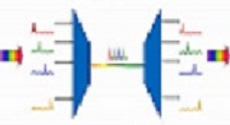
\includegraphics[scale=1.2]{iapam.jpg}
    \caption{multiplexação FDM/TDM}
    \label{fig:imagem}
     \ref{fig:imagem} 
\end{figure}

\section{Relevância}
\label{rel}
\label{dois}

A tecnologia é um dos alicerce do novo século. Se antigamente não era tão popularizado, havia uma abrangência menor para que não vinhesse a ser tão frequente naquele tempo. Hoje, redes de computadores é algo tão comum, tão usado em vários ambientes em geral, facilitando uma demanda maior de profissionais na busca de emprego nessa área.\cite{rel}\cite{dois}

\section{Relação Interdisciplinares}
\label{revinterd}
\label{tres}

\begin{table}[h]
 \centering
 {\renewcommand\arraystretch{1.25}
  \caption{Outras disciplina > Relações}
 \begin{tabular}{ l l }
  \cline{1-1}\cline{2-2}  
   
  \\  
  \cline{1-1}\cline{2-2}  
    \multicolumn{1}{|p{3.850cm}|}{\textbf{IF685 - Gerenciamento de dados e Informação}} &
    \multicolumn{1}{p{4.217cm}|}{‘A disciplina ofertada pelo curso aborda a base sólida de banco de dados, abrangendo recursos de modelagem até recursos de linguagem atuais.\cite{tres}}
  \\  
  \cline{1-1}\cline{2-2}  
    \multicolumn{1}{|p{3.850cm}|}{\textbf{IF - 678 Infra-estrutura de Comunicação}} &
    \multicolumn{1}{p{4.217cm}|}{Essa cadeira é uma complementação de redes de computadores, onde o aluno passa a entender os diversos aspectos e implementar toda estrutura de redes. Além disso, a disciplina trás um pouco da história e como a camada de rede é estruturada. \cite{revinterd}}
  \\  
  \hline

 \end{tabular} }
\end{table}

\section{Referência}
\bibliographystyle{plain}
\bibliography{iapam}
\end{document}
